\clearpage{\pagestyle{empty}\cleardoublepage}
\chapter{Visualizzazione di dati riguardanti la Sostenibilità} %crea il capitolo
%%%%%%%%%%%%%%%%%%%%%%%%%%%%%%%%%%%%%%%%%imposta l'intestazione di pagina
\lhead[\fancyplain{}{\bfseries\thepage}]{\fancyplain{}{\bfseries\rightmark}}
\pagenumbering{arabic}                  %mette i numeri arabi
\section{Introduzione al tema della Sostenibilità}
\noindent L'enciclopedia Treccani 
riporta la seguente definizione per la parola ``Sostenibilità":
\textit{``Nelle scienze ambientali ed economiche, condizione di uno sviluppo in grado di assicurare il soddisfacimento dei bisogni della generazione presente senza compromettere la possibilità delle generazioni future di realizzare i propri \cite{treccani}."}\newline\newline
È stata l'Organizzazione delle Nazioni Unite (Figura \ref{onuImg}), più comunemente denominata ONU a fare suo questo termine e a crearne la definizione.\newline
Il primo vero e proprio concetto di ``sostenibilità" emerse infatti dalla prima conferenza ONU riguardante l'ambiente nel 1972 \cite{stoccolma}.\newline
\begin{figure}[H]
    \centering
    
\includegraphics[width=0.3\linewidth]{img/onu.jpg}
    \caption{Logo dell'Organizzazione delle Nazioni Unite (ONU) \cite{onuImg}}
    \label{onuImg}
\end{figure}
\noindent Solo successivamente però verrà definito con più chiarezza cosa si intende con ``sostenibilità" o 
``sviluppo sostenibile".\newline
\subsection{La Storia della Sostenibilità}
\noindent Nel 1987, Gro Harlem Brundtland, presidente della Commissione mondiale su Ambiente e Sviluppo presenta il rapporto \textit{``Our common future"}.\newline
Il rapporto constatava come la causa di una buona parte dei problemi mondiali fosse causato dall'enorme differenza di ricchezza tra la zona settentrionale e meridionale nel pianeta.\newline
Quasi tutti i paesi a sud vivevano una condizione molto grave di povertà mentre quelli a nord non riuscivano a rispettare modelli di produzione sostenibili.\newline
Il rapporto è dunque di enorme rilevanza, in quanto evidenzia la necessità di agire per bilanciare la situazione di entrambi i lati del pianeta \cite{ourCommon}.\newline
Le linee guida presenti sul rapporto sono ancora oggi valide e da tenere in considerazione.\newline
La conferenza più sensazionale sull'argomento ``ambiente" fu in ogni caso quella del 1992, a Rio de Janeiro.\newline
All'evento che prese il nome di \textit{Conferenza sull'ambiente e lo sviluppo delle Nazioni Unite} (o UNCED, ma fu anche chiamato \textit{Summit della terra}) parteciparono 172 rappresentanze governative (tra le quali 108 Capi di Stato) e 2.400 rappresentanti di organizzazioni non governative. Circa 17.000 persone partecipano al Forum delle ONG.\newline
I temi trattati furono:
\begin{itemize}
    \item la scarsità di acqua sul pianeta;
    \item le limitazioni di sostanze tossiche nei modelli di produzione;
    \item il rimpiazzamento dei combustibili fossili con risorse di energia alternative;
    \item la riduzione delle emissioni e dello smog causato dai veicoli, specialmente nelle grandi città e nelle metropoli.
\end{itemize}
Furono redatti al termine della conferenza 5 documenti fondamentali che costituiranno le linee-guida per l'azione di tutti gli Stati membri:
\begin{enumerate}
    \item \textbf{UNFCCC (Convenzione quadro delle Nazioni Unite per i cambiamenti climatici)}\newline
Si tratta di un trattato internazionale il cui scopo è combattere con una serie di mezzi, di scelte politiche e di decisioni collettive il grande problema del cambiamento climatico.
    \item \textbf{La Convenzione sulla diversità biologica}\newline
    Entrata in vigore nel 1993 il suo scopo è la conservazione della diversità biologica.\newline
    Il documento tratta anche l'uso sostenibile dei componenti della diversità biologica e l'equa suddivisione dei benefici provenienti dall'uso delle risorse genetiche.
    \item \textbf{Agenda 21}\newline
    In questa agenda compaiono numerose proposte al fine di affrontare vari problemi sociali ed economici prima dell'arrivo del nuovo secolo. I temi trattati sono molteplici; si parla di combattere la povertà, di proteggere l'atmosfera, gli alberi, le foreste, gli ecosistemi etc.\newline 
    Molto simili sono gli Obiettivi di Sviluppo Sostenibile che sono stati fissati come traguardi da raggiungere entro il 2030. L'argomento verrà trattato con cura nella sottosezione \ref{sub:sdg}.
    \item \textbf{La Dichiarazione di Rio su Ambiente e Sviluppo}\newline
    La Dichiarazione di Rio è il documento che definisce tutti i diritti e le responsabilità degli Stati membri rispetto agli obiettivi imposti.
    \item \textbf{I Principi sulle Foreste}\newline
    Nel documento ``I Principi sulle foreste" viene riconosciuto per la prima volta come estremamente vitale ed importante il lavoro svolto dalle foreste non solo per l'ambiente, ma anche per l'economia mondiale e il benessere di tutti. 
\end{enumerate}
\noindent Nel Settembre del 2000 fu firmata dalle Nazioni Unite la \textit{Millenium Declaration}. Dalla dichiarazione emersero gli Obiettivi di Sviluppo del Millennio (Millennium Development Goals o MDG), ovvero degli obiettivi imposti dall'ONU che tutti i 193 stati membri si sono impegnati a raggiungere per l'anno 2015).
\begin{figure}[H]
    \centering
  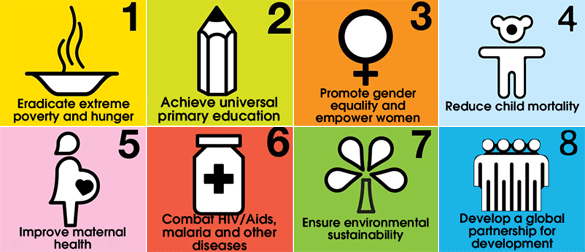
\includegraphics[width=\linewidth]{img/mdgs.png}
  \caption{Millennium Development Goals \cite{mdgImg}}
\end{figure}
\noindent Gli MDG si impegnavano a:
\begin{enumerate}
    \item Cancellare la povertà estrema e la fame nel mondo;
    \item Rendere universale l'istruzione primaria;
    \item Promuovere la parità dei sessi;
    \item Ridurre la mortalità infantile;
    \item Migliorare la sanità materna;
    \item Combattere l'HIV, l'AIDS, la malaria e altre malattie;
    \item Garantire la sostenibilità ambientale;
    \item Creare un'alleanza mondiale per lo sviluppo.
\end{enumerate}

\noindent Nel 2012 l'ONU scelse nuovamente Rio de Janeiro come sede per la Conferenza sullo sviluppo sostenibile. L'evento venne denominato \textit{``Rio 2012"} o \textit{``Rio+20"}.
Durante la conferenza si discusse a lungo riguardo all'idea di istituire degli SDG (Sustainable Development Goals).
La soluzione che si raggiunse è racchiusa nel documento ``Future We Want" (Il futuro che vogliamo) \cite{futureWeWant}.\newline
Il documento tratta dei consueti temi  come origini dell'energia, sanità, bontà dell'acqua.
La conferenza di Rio+20 non definì obiettivi concreti come accadde per esempio con il rilascio dell'Agenda 21.\newline
Quel che si sapeva, era che gli obiettivi sarebbero dovuti essere pochi o comunque in numero limitato, facili da capire, semplici da comunicare.
Per la creazione degli obiettivi fu istituito dunque \textit{Open Working Group (OWG)}, un gruppo di 30 membri il cui compito sarebbe stato preparare proposte per i cosiddetti SDG \cite{owg}.
\subsection{Gli obiettivi di Sviluppo Sostenibile}
\label{sub:sdg}
\noindent OWG selezionò dunque diciassette obiettivi principali, che prendono il nome di Sustainable Development Goals, o SDG.
Ogni singolo SDG ha carattere universale, è rivolto a tutti i paesi, indipendentemente dalle rispettive situazioni economiche.
Gli SDG sono obiettivi comuni. Tutti i paesi e le nazioni del mondo dovrebbero essere interessate al loro raggiungimento.\newline
Gli SDG sono stati pensati come sostituti degli MDG per l'intervallo di tempo che va dal 2015 al 2030 \cite{bureau}.\newline
A causa dell'epidemia di Covid-19 dell'anno 2020 molti obiettivi hanno subito ingenti rallentamenti. 
\begin{figure}[H]
  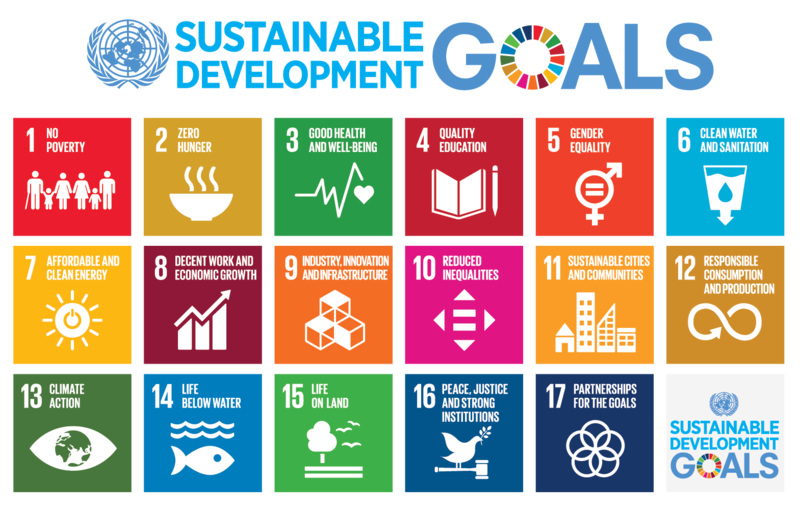
\includegraphics[width=\linewidth]{img/goals.png}
  \caption{Sustainable Development Goals \cite{sdgImg}}
\end{figure}

\noindent Viene di seguito riportata la lista degli SDG insieme alla loro introduzione ufficiale ed una breve descrizione degli obiettivi.
\begin{enumerate}
\item \textbf{Povertà Zero}\newline
\textit{``Porre fine alla povertà in tutte le sue forme, ovunque \cite{goals}."}\newline
Il goal tratta il problema della povertà. Lo scopo è sradicarla completamente dalla società, eliminandola per sempre. Entro il 2030 la povertà nel mondo sarebbe dovuta calare al 6\% considerando tutta la popolazione mondiale. Sfortunatamente la pandemia globale di COVID-19 dell'anno 2020 pare aver rallentato notevolemente il processo \cite{reportONU}.
\item \textbf{Fame Zero}\newline
\textit{``Porre fine alla fame, garantire la sicurezza alimentare migliorare nutrizione e promuovere l’agricoltura sostenibile \cite{goals}."}\newline
Nel 2018 una persona su nove nel mondo è denutrita. \cite{stateOfFood}\newline
Lo scopo di questo SDG è aumentare la produttività agricola, favorendo l'economia delle piccole imprese che fanno parte del settore. Anche in questo caso, la forte crisi mondiale causata dalla pandemia del 2020 ha peggiorato ulteriormente la situazione, già molto grave a causa dei rapidi cambiamenti climatici nel mondo.
\item \textbf{Buona salute e benessere per le persone}\newline
\textit{``Garantire una vita sana e promuovere il benessere di tutti a tutte le età \cite{goals}."}\newline
Sensibilmente più generico dei primi due, il terzo obiettivo punta al miglioramento generale della sanità. Temi principali di questo SDG sono la diminuzione dei tassi di mortalità, la ricerca di cure e rimedi a malattie (quali anche HIV/AIDS) o anche trovare modi per favorire l'accesso all'acqua potabile a chiunque nel mondo.
\item \textbf{Educazione paritaria e di qualità}\newline
\textit{``Promuovere un'educazione di qualità, inclusiva e paritaria e garantire opportunità di apprendimento permanente per tutti \cite{goals}."}\newline
Scopo di questo SDG è combattere l'analfabetizzazione.\newline
Il principale obiettivo di questo obiettivo è garantire un'educazione di livello primario e secondario libera, paritaria e di buona qualità per tutti i bambini del mondo.
\item \textbf{Parità di genere}\newline
\textit{``Raggiungere la parità di genere ed emancipare tutte le donne e le ragazze \cite{goals}."}\newline
In numerosi stati, per l'esattezza centoquarantatre, il diritto di uguaglianza tra generi diversi è presente nelle relative Costituzioni, compresa l'Italia che lo cita nell'articolo tre \cite{italianCostitution}.\newline
A differenza degli altri obiettivi questo tratta un problema di tipo completamente sociale.
\item \textbf{Acqua pulita e servizi igienico-sanitari}\newline
\textit{``Garantire a tutti l'accessibilità e la gestione sostenibile dell'acqua e dei servizi igienico-sanitari \cite{goals}."}\newline
Tema centrale in questo caso è l'acqua.
Lo scopo di questo SDG è riuscire a fornire a chiunque acqua potabile e l'accesso a sistemi igenici-sanitari.
\item \textbf{Energia pulita e accessibile}\newline
\textit{``Garantire a tutti l'accesso a servizi energetici economici, affidabili, sostenibili e moderni \cite{goals}."}\newline
Scopo di questo SDG è migliorare l'efficienza energetica preferendo metodi sostenibili come carburanti e tecnologie che non inquinino a discapito dei combustibili fossili. L'accessibilità a questi mezzi dovrebbe inoltre essere garantita a tutti.
\item \textbf{Lavoro dignitoso e crescita economica}\newline
\textit{``Promuovere una crescita economica inclusiva, sostenuta e sostenibile, un’occupazione piena e produttiva e un lavoro dignitoso per tutti \cite{goals}."}\newline
Questo obiettivo è principalmente stato pensato per i paesi del quarto mondo.
Ogni anno il 7\% del PIL dovrebbe essere destinato ai paesi più poveri.
Tema centrale è anche la disoccupazione giovanile.
\item \textbf{Industria, Innovazione e Infrastruttura}\newline
\textit{``Costruire infrastrutture resilienti, promuovere un’industrializzazione inclusiva e sostenibile e favorire l’innovazione \cite{goals}."}\newline
Uno degli obiettivi più duramente colpiti dalla crisi alimentata dalla pandemia di COVID-19 del 2020.
Lo scopo è aumentare l'industrializzazione per combattere la crisi nei paesi più poveri usando metodi sostenibili.
\item \textbf{Ridurre le disuguaglianze}\newline
\textit{``Ridurre le diseguaglianze economiche dentro e fuori i confini nazionali \cite{goals}."}\newline
Introduciamo il Coefficiente di Gini: un indice per la misura della disuguaglianza della distribuzione del reddito.
Valori vicini allo 0 indicano una situazione in cui il denaro è distribuito in maniera uniforme tra i cittadini mentre valori vicini a 1 indicano la situazione opposta, ovvero poche persone posseggono la maggior parte del denaro \cite{gini}.\newline
Fine di questo obiettivo è ottenere valori vicini allo 0 nella maggior parte dei paesi, specialmente in quelli più poveri.
\item \textbf{Città e comunità sostenibili}\newline
\textit{``Rendere le città e gli insediamenti urbani inclusivi, sicuri, resilienti e sostenibili \cite{goals}."}\newline
Garantire a chiunque un'abitazione a prezzi modici è lo scopo di questo SDG. Tema principale è anche l'eliminazione delle baraccopoli, che risulterebbe in un'ulteriore miglioramento della sanità pubblica.
\item \textbf{Consumo e produzione responsabile}\newline
\textit{``Garantire modelli sostenibili di produzione e di consumo \cite{goals}."}\newline
Combattere lo spreco è la finalità principale di questo obiettivo.\newline Preferire l'uso di materiali riciclati e aumentare le percentuali di riciclaggio nazionali sono strumenti utili per raggiungere questo scopo.
\item \textbf{I cambiamenti del clima}\newline
\textit{``Si devono adottare misure urgenti per contrastare il cambiamento climatico e i suoi impatti regolando le emissioni e promuovendo gli sviluppi nell'energia rinnovabile \cite{goals}."}\newline
Tema principale del nostro secolo è proprio il riscaldamento globale. Ogni paese dovrebbe avere un piano per la riduzione dei rischi dovuti ai cambiamenti climatici, mentre solo ottantacinque ne hanno uno. L'argomento verrà anche approfondito nella sottosezione \ref{sub:climateChange}.
\item \textbf{Vita sott'acqua}\newline
\textit{``Preservare e usare in modo sostenibile gli oceani, i mari e le risorse marine per lo sviluppo sostenibile \cite{goals}."}\newline
I mari e gli oceani ricoprono circa il 70\% della superficie terrestre. L'inquinamento causato dal rilascio della plastica e di altre sostanze prodotte dagli umani sta irrimediabilmente distruggendo numerosi ecosistemi marini. L'acidità del mare potrebbe salire di oltre il 100\% entro i prossimi ottanta anni, causando problemi in più della metà della vita sott'acqua \cite{sdgs}.\newline
Preservare gli oceani è lo scopo di questo SDG.
\item \textbf{Vita sulla terra}\newline
\textit{``Proteggere, recuperare e promuovere l'uso sostenibile degli ecosistemi terrestri, gestire in modo sostenibile le foreste, combattere la desertificazione, arrestare il degrado del suolo e fermare la perdita della biodiversità \cite{goals}."}\newline
Complementare al precedente obiettivo, questo si occupa di preservare la vita sulla terra, richiedendo più attenzione per evitare l'estinzione di numerose specie di animali.\newline Preservare l'ordine naturale del mondo sulla terra in tutte le sue forme è lo scopo di questo SDG.
\item \textbf{Pace, giustizia e istituzioni forti}\newline
\textit{``Promuovere società pacifiche e solidali per lo sviluppo sostenibile, garantire l'accesso alla giustizia per tutti e costruire istituzioni efficaci, responsabili e solidali a tutti i livelli \cite{goals}."}\newline
Un'ulteriore SDG puramente in ambito sociale è il penultimo. Le finalità sono ridurre il tasso di criminalità ed aumentare la giustizia creando, migliorando o potenziando leggi per vivere in un mondo più pacifico e giusto.
\item \textbf{Partnership per gli obiettivi}\newline
\textit{``Rafforzare le modalità di attuazione rilanciare il partenariato globale per lo sviluppo sostenibile \cite{goals}."}\newline
In questo SDG si chiede la collaborazione di ogni stato del mondo per raggiungere tutti gli obiettivi precedentemente elencati. L'aiuto dei paesi più ricchi è molto rilevante e quasi vitale per quanto riguarda la crescita economica dei più poveri.
\end{enumerate}
\subsection{La sfida del millennio: il Riscaldamento Globale}
\noindent Dalla rivoluzione industriale, sono stati rilasciati oltre 1,5 trilioni di tonnellate di anidride carbonica nell'atmosfera terrestre. 
Nel 2019 le emissioni continuavano ad essere circa 37 miliardi in più. 
Si tratta di numeri spaventosi, rispetto all'anno 2000 il valore è cresciuto di circa il 50\%.\newline
Questi valori sono relativi solo alla CO$_2$. Le emissioni di ogni giorno contengono anche volumi crescenti di altri gas quali metano e protossido di azoto. Se combiniamo tutti i gas serra, ogni anno vengono emesse circa 51 miliardi di tonnellate di equivalenti di biossido di carbonio.\newline
L'unico modo per ripristinare un clima naturale e limitare i danni causati è ridurre le emissioni dei gas serra, rapidamente.\newline
Nonostante però tutti i paesi del mondo siano concordi sul fatto che il riscaldamento globale sia un problema collettivo non si riescono a trovare accordi stabili su come affrontare il problema \cite{whosResponsible}.\newline
Nel 2017, le emissioni sono state, contando solo CO$_2$, circa 36 miliardi di tonnellate. Il 53\% di esse proviene dall'Asia, il 18\% dal Nord America e il 17\% dall'Europa. Solo la Cina ha emesso circa il 27\% delle emissioni totali per quell'anno, seguita dagli USA che ne hanno emessi il 15\% e l'Unione Europea che ne ha prodotte il 10\%.\newline
Solo Cina, USA e UE emettono più del 50\% delle emissioni globali in questi anni. È molto importante per queste tre potenze mondiali trovare un accordo per combattere il cambiamento climatico il prima possibile, o le conseguenze sarebbero disastrose \cite{co2Green}.
Degli scorsi 22 anni, 20 hanno raggiunto temperature record mai viste prima \cite{wmo}.
I paesi più ricchi hanno le risorse e tecnologie in grado di sviluppare soluzioni a basso costo per limitare le emissioni di carbonio e diffonderle in tutto il mondo.
È necessario che la tecnologia a basse emissioni di carbonio diventi più economica, altrimenti i paesi più poveri diventerebero dipendenti da emisisoni di CO$_2$.
Fortunatamente il costo delle energie rinnovabili sta diminuendo negli anni, ma è un processo che sta avvenendo troppo lentamente. \newline
Il cambiamento climatico è un problema globale e nessun paese può risolverlo da solo.\newline
Capire chi è il principale responsabile non è semplice come sembra ed è una domanda insensata e banale da porsi.
In realtà per risolvere il problema ogni stato dovrebbe semplicemente impegnarsi e fare del suo meglio \cite{whosResponsible}.

\label{sub:climateChange}
\section{Data Visualization}
\noindent Con il termine Data Visualization si intende una rappresentazione grafica di dati e informazioni. Usare elementi come grafici o mappe per rappresentare fenomeni o concetti rende più semplice la comprensione degli stessi all'utente a cui vengono presentati \cite{dataVisual}.
\subsection{Concetti di Base per la visualizzazione di Dati}
\noindent I nostri occhi sono attratti da quello che potremmo definire un ``pattern". Può risultare più semplice capire quando due colori sono diversi, o quando una figura geometrica rappresenta un cerchio invece di un quadrato \cite{dataVisual}.\newline
I dati che si vogliono presentare possono essere di due tipi: strutturati o destrutturati.\newline
\noindent Con dati strutturati intendiamo un set di dati che rispetta un certo schema di regole preimpostato \cite{strucData}.\newline
Ad esempio le entry di un DataBase sono dati di tipo strutturato perché la struttura delle tabelle è scelta in anticipo rispetto all'inserimento dei dati. Al momento di inserire una nuova entry è necessario rispettare la struttura presente.\newline\newline
I dati destrutturati al contrario non hanno un modello o un dominio predefinito \cite{strucData}.\newline
Ad esempio un'immagine a colori o un file audio sono ottimi esempi per rappresentare un tipi di dati non strutturati. Non è infatti possibile estrapolare informazioni utili e sensate usando le stesse metologie usate nei dati strutturati.\newline
Rappresentare dati non strutturati è ovviamente molto più complicato. In questa tesi verrà trattata solo la visualizzazione di dati fortemente strutturati.\newline
\noindent Con Data Visualization intendiamo una forma di arte visiva.
Grazie ai grafici è possibile estrapolare un numero impressionante di informazioni da un determinato DataSet.

\subsection{Best Practice, come presentare efficacemente i Dati}
\noindent Riuscire a rappresentare i dati in modo che siano comprensibili e semplici da capire non è semplice. Ci sono tuttavia numerose tecniche che se si possono utilizzare per semplificare la Data Visualization.

\begin{itemize}
    \item \textbf{Conoscere gli utenti a cui è rivolta la presentazione dei Dati}
    Domande fondamentali da porsi sono ``Cosa interessa alle persone a cui sono rivolti questi dati? Cosa vogliono vedere? Quale messaggio devono recepire?"\newline
    La tipologia di utenza a cui è rivolta la visualizzazione dei dati è un tassello fondamentale da tenere a mente durante la progettazione dei grafici.\newline
    Il modo in cui vengono capiti e recepiti i dati varia anche da persona a persona, in base al mestiere, alla cultura, all'età.\newline
    Mettersi nei panni degli utenti che visualizzeranno i dati è una buona idea per creare diagrammi semplici da capire \cite{oracle}.
    \item \textbf{I dati devono essere chiari}\newline
Esistono svariati tipi di dati, strutturati, destrutturati, interi, categorici.
Alcuni grafici sono più utili di altri per la rappresentazione di determinati tipi di dato.\newline Ecco una breve descrizione delle tipologie di dati più comuni:
\begin{enumerate}
    \item \textbf{Dati Ordinali}: I dati hanno una sequenza logica, nel tempo o come concetti, per esempio la classifica di un torneo rappresenta un esempio di tipi di dati ordinali.
    \item \textbf{Dati Categorici}: Il dominio dei dati è limitato ad un numero finito di valori che possono assumere. Il continente in cui può avvenire un determinato evento per esempio è un tipo di dato categorico in quanto anche il numero di continenti nel mondo è finito.
    \item \textbf{Dati quantitativi}: Sono dati numerici, indicano il valore di qualcosa utilizzando una scala numerica. Alcuni esempi possono essere un vestito che costa 40 euro, una giornata in cui la temperatura massima è 34C\degree.
\end{enumerate}
Alcuni tipi di grafici sono più indicati per determinati tipi di dato. Per esempio, un grafico a dispersione (scatter plot) funziona meglio su entry con dati di tipo quantitativo.
In figura \ref{iceCream} è rappresentato un grafico a dispersione che prova a mettere in correlazione la temperatura esterna e i guadagni dati dalla vendita di gelati.
\begin{figure}[H]
    \centering
    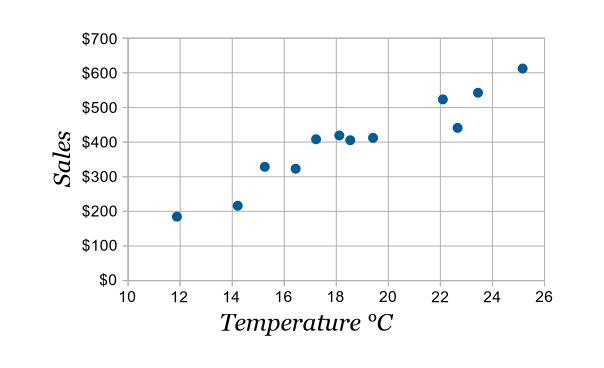
\includegraphics[width=0.9\linewidth]{img/iceCream.png}
    \caption{Grafico a dispersione: correlazione tra vendite di gelati e temperatura esterna \cite{mathsin}}
    \label{iceCream}
\end{figure}
\noindent Notiamo come si capisca perfettamente che all'aumentare della temperatura aumenta anche il fatturato.\newline
La scelta del grafico è risultata adatta perché il nostro occhio riconosce un pattern simile a una linea tra i punti del grafico.\newline
In altre parole, arriva forte e chiaro il messaggio c'è un qualche tipo di correlazione \cite{mathsin}.
    \item \textbf{Scegliere bene il tipo di Dashboard}\newline
Selezionare la struttura con cui vogliamo rappresentare i dati è una delle parti più importanti per non confondere l'utente quando guarda lo schermo. Esistono principalmente tre tipi di dashboard:
\begin{enumerate}
    \item \textbf{DashBoard Analitica}: Questo tipo di dashboard viene utilizzata principalmente per rappresentare numerose viste su un solo e unico argomento centrale \cite{klipfolio};
    \item \textbf{DashBoard Strategica/Esecutiva}: La dashboard strategica o esecutiva viene utilizzata per mostrare soprattutto le variazioni degli indicatori chiave di prestazione (ICP o KPI). Si tratta di indici che monitorano l'andamento di processi aziendali \cite{klipfolio};
    \item \textbf{DashBoard Operazionale}: Come la dashboard strategica, la dashboard operazionale nasce per mostrare dati relativi a indici aziendali. La differenza rispetto agli altri tipi di dashboard però è che i dati vengono aggiornati molto più frequentemente, per natura dei dati stessi \cite{klipfolio}.
\end{enumerate}
La scelta della dashboard è quindi molto importante non solo per quanto riguarda la scelta del design da utilizzare. Il tipo di struttura su cui essa si basa deve essere scelto con cura durante la fase di progettazione, per fare in modo che il sistema risulti affidabile \cite{oracle}.
\end{itemize}

\subsection{Utilizzo di Infografiche, l'importanza del Design}
\noindent Il Dizionario di Oxford definisce un'infografica come ``una rappresentazione visuale per mostrare un informazione o dei dati \cite{oxofordDictionary}."\newline
Un'infografica è una collezione di immagini, di grafici, di scritte che offrono un modo più semplice per comprendere un determinato argomento.
Alcune ricerche mostrano come il volume di ricerca per il tema ``Infografiche" è aumentato di oltre 800\% tra il 2010 e il 2012 \cite{martech}.\newline
Anche a causa di questa spaventosa crescita di interesse nei confronti dell'argomento, numerose infografiche che circolano sul web sono di pessima fattura e poco efficaci.
Infografiche con un design fatto male possono distorcere le informazioni che si desiderano trasmettere invece che enfatizzarle.
Creare un'infografica efficiente e carina richiede la conoscenza di alcune tecniche base di design.
L'uso di template già pronti è assolutamente raccomandato, ma è importante scegliere con cura quale usare in base all'argomento trattato.
Analizziamo la Figura \ref{infographExample}, rappresentante un esempio di un'infografica.
\begin{figure}[H]
    \centering
    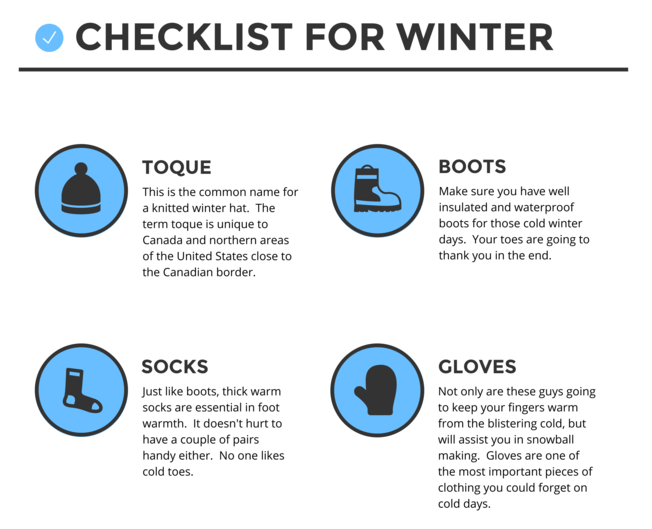
\includegraphics[width=0.9\linewidth]{img/infograpExample.png}
    \caption{Esempio di un'infografica \cite{venngage}.}
    \label{infographExample}
\end{figure}
\noindent Il titolo è la scelta dei colori ci aiutano a capire facilmente quale sia lo scopo finale. Si tratta di una lista di oggetti da procurarsi per l'inverno.\newline
La scelta di colori spenti ci aiuta a identificare meglio la stagione come \textit{``inverno"} in quanto siamo da sempre familiare al fatto che d'inverno tutto si spegne, si congela. Da sempre siamo abituati a pensare al blu e all'azzurro come colori freddi, infatti anche sui rubinetti di casa usiamo il colore blu per indicare l'acqua fredda.
Cosa succederebbe se cambiassimo il colore? Perderemmo un'informazione importante e di conseguenza potremmo disorientare l'utente e non far recepire il messaggio.\newline
Anche l'inserimento di icone ed immagini nell'infografica è fondamentale.\newline
Un'immagine è molto più rappresentativa di un concetto di una scritta, inoltre è anche più facilmente identificabile anche da lontano. Se rimuovessimo le immagini dall'infografica la renderemmo spoglia, non diversa da un libro o da un comune documento.
Alcune ricerche mostrano come i colori e le forme giochino un ruolo fondamentale quando si tratta di attirare l'attenzione delle persone \cite{facebook}.\newline
Alcuni concetti chiave quando si tratta di creare un buon design per le infografiche sono:
\begin{itemize}
    \item \textbf{Scelta del Titolo}: scegliere un buon titolo può risultare molto utile. Si sfrutta lo stesso principio che si usa nei giornali. I titoli devono essere chiari e accattivanti, in questo modo sarà più facile attirare l'attenzione \cite{venngage};
    \item \textbf{Simmetria}: la simmetria attira l'attenzione perché emana perfezione. Tabelle, schemi simmetrici, argomenti incapsulati in sezioni di determinate forme geometriche sono ottimi elementi per infografiche \cite{venngage};
    \item \textbf{Usare efficientemente i colori}: l'uso dei colori è fondamentale. Alcuni colori si sposano meglio tra loro. Solitamente si sceglie uno schema di colori su cui basare l'intera infografica e non se ne usano altri. Troppi colori causano confusione \cite{venngage};
    \item \textbf{Consistenza}: il design deve essere consistente. Il font usato, i colori, lo stile delle immagini non possono subire cambiamenti troppo drastici durante la creazione dell'infografica. La semplicità ripaga \cite{venngage}.
\end{itemize}
\section{Interactive Public Ambient Display}
\noindent In questo capitolo verrà trattato il tema dell'Interactive Public Ambient Display.
Si tratta di una tecnologia in fase di sviluppo che mira all'inserimento di schermi in zone urbane o comunque densamente popolate, utilizzabili da chiunque, in grado di mostrare informazioni agli utenti che vi interagiscono, sia che siano esse pubbliche o private.\newline
Alcuni esempi di prototipi per ora sono in grado di mostrare le attività da svolgere durante la giornata, le note, gli appunti o addirittura messaggi.\newline
Realizzare questi sistemi tuttavia offre anche alcune sfide interessanti. Come si può mantenere la privacy degli utenti? Come possiamo far sentire l'utente che usa il sistema a proprio agio? \cite{intVideo}\newline 
\subsection{Le fasi dell'iterazione tra Utenti e Sistemi}
\noindent Il Display si comporta in maniera differente in base a come l'utente lo approcia, in particolare le fasi delle iterazioni che l'utente può avere con il sistema sono quattro:
\begin{enumerate}
    \item \textbf{Ambient Display}: Ci troviamo in un ambiente neutrale in cui l'utente riesce ad ottenere solo informazioni generiche dal Display;
    \item \textbf{Interazione Implicita (Subtle Interaction)}: L'utente comincia ad avvicinarsi al Display il quale comincia a riconoscere i suoi movimenti. In questa fase il Display può anche mostrare se ci sono notifiche urgenti per lo specifico utente che si avvicina. Non c'è ancora una vera e propria iterazione tra utente e sistema;
    \item \textbf{Interazione Sottile (Implicit Interaction)}: L'utente in questa fase si trova proprio davanti allo schermo. Cominciano a comparire sullo schermo informazioni più sensibili, per esempio il numero di appuntamenti che si hanno in quel determinato giorno. La durata media di questa fase è di circa un minuto;
    L'iterazione con lo schermo avviene utilizzando principalmente la posizione del corpo, delle braccia e delle gambe;
    \item \textbf{Interazione Personale (Personal Interaction)}: L'utente accede ad un area più personale e privata solo tramite l'ultima fase. Se nella fase di Iterazione Sottile si seleziona principalmente un'azione da svolgere, tramite questa ultima fase si sceglie il ``cosa fare" nello specifico.\newline
    Si tratta di un'area privata e strettamente legata all'utente, per questo l'iterazione avviene molto vicina allo schermo ed utilizzando movimenti delle mani o anche direttamente il touch screen.
\end{enumerate}

\noindent In figura \ref{fig:phasesStages} viene riportata la rappresentazione grafica delle quattro fasi.

\begin{figure}[H]
    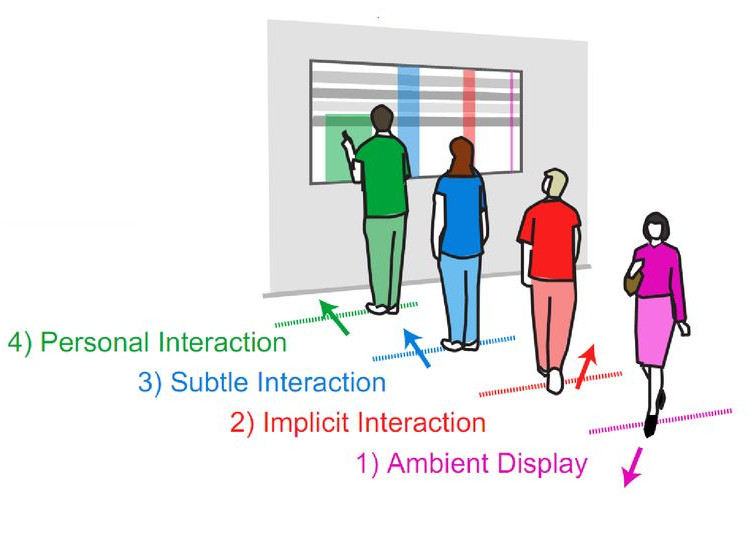
\includegraphics[width=\linewidth]{img/publicToPersonal.jpg}
    \caption{Iterazioni degli utenti con Interactive Public Ambient Display \cite{interactive}}
    \label{fig:phasesStages}
\end{figure}
\noindent In figura \ref{fig:phasesStates} viene invece riportato il diagramma degli stati per il passaggio tra fasi. Una fase può trovarsi in più stati in base alla posizione che assume l'utente davanti al Display. Per esempio l'Interazione Sottile contiene due stati: l'utente potrebbe star semplicemente osservando le sue notifiche \textit{(OVERVIEW)} oppure potrebbe star scegliendo un elemento con cui interagire \textit{(SELECT)}. Gli eventi del diagramma sono principalmente movimenti che l'utente effettua davanti allo schermo \cite{interactive}.

\begin{figure}[H]
     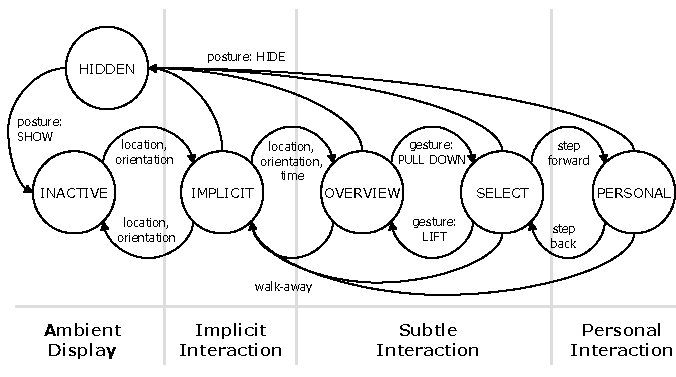
\includegraphics[width=\linewidth]{img/stateDiagram.png}
     \caption{Diagramma degli stati delle iterazioni \cite{interactive}}
     \label{fig:phasesStates}
\end{figure}

\subsection{Principi e Design, come attirare l'attenzione degli utenti}
\noindent Quando si crea un sistema di tipo Interactive Public Ambient Display è necessario seguire alcune linee guida per il buon funzionamento:

\begin{itemize}
    \item \textbf{Grafiche tranquille e non troppo elaborate}\newline
 Se l'ambiente che viene offerto risulta troppo visivamente complicato o confusionario il numero di utenti disposti ad usare il Display potrebbe calare drasticamente. È importante mantenere una certa semplicità nella scelta del design \cite{interactive};
    \item \textbf{Comprensibilità}\newline
I messaggi che si vogliono mostrare devono essere comprensibili. Non importa se le informazioni non sono da subito semplici da capire, l'importante è che l'utente riesca a comprendere cosa gli viene presentato prima che se ne vada \cite{interactive};
    \item \textbf{Sistemi di notifica}\newline
 Le notifiche sono il meccanismmo alla base dei sistemi di tipo Interactive Public Ambient Display. È molto importante avvertire l'utente se ci sono notifiche mantenendo un livello di privacy adeguato in base al tipo di notifica e al tipo di utente \cite{interactive};
    \item \textbf{Iterazioni brevi e fluide}\newline
    Il mondo di oggi è molto caotico e il tempo è una componente fondamentale della vita di chiunque. A nessuno piace perdere tempo. Ogni singola iterazione che l'utente effettua sul Display deve essere rapida ma comunque gradevole all'occhio. Troppa lentezza fa perdere interesse, troppa velocità causa un senso di agitazione \cite{interactive};
    \item \textbf{Usabilità Immediata}\newline
    Non deve essere richiesto alcun tipo di conoscenza pregressa per usare il Display. L'utente dovrebbe essere in grado di usare il sistema senza difficoltà anche la prima volta che vi entra in contatto \cite{interactive};
    \item \textbf{Uso combinato}\newline
    Se il Display che ospita il sistema è molto grande probabilmente più utenti vorranno provarlo allo stesso tempo \cite{interactive};
    \item \textbf{Privacy}\newline
    Non per tutti potrebbe risultare facile utilizzare un Display pubblico per accedere ai propri dati, inoltre informazioni che potrebbero sembrare estremamente sensibili per determinate tipologie di persone potrebbero non esserlo affatto per altre. Se l'utente desidera nascondere delle notifiche prefissate o messaggi di un certo tipo deve avere la possibilità di farlo \cite{interactive}.
\end{itemize}


